% \section{Resultados de las ejecuciones de los algoritmos de búsqueda}
% A continuación se muestra el valor de la función objetivo para cada uno de los distintos algoritmos ejecutados y el tiempo de ejecución final.
% \subsection{Artículos}
% \Solucion {}
% {
% \begin{description}
% 	\item[alg\_1] \texttt{PAC(Efficient C-HAC/Selección de paquetes proporcional)}
% 	\item[alg\_2] \texttt{PAC(Efficient C-HAC/Selección de paquetes)}
% 	\item[alg\_3] \texttt{PAC(BOBO-10/Selección de paquetes proporcional)}
% 	\item[alg\_4] \texttt{PAC(BOBO-10/Selección de paquetes)}
% 	\item[alg\_5] \texttt{PAC(BOBO-160/Selección de paquetes proporcional)}
% 	\item[alg\_6] \texttt{PAC(BOBO-160/Selección de paquetes)}
% 	\item[alg\_7] \texttt{PAC(BOBO-ex/Selección de paquetes proporcional)}
% 	\item[alg\_8] \texttt{PAC(BOBO-ex/Selección de paquetes)}
% \end{description}
% }
% {$\in$ $(0,1; 0,3; 0,5; 0,7; 0,9)$}
% {10}
% {5}
% A continuación se muestran los valores de la función objetivo obtenidos:\\
% \begin{table}[H]
% \centering
%   \resizebox{\textwidth}{!} {
%     \begin{tabular}{|lc|cccc|}
%     \hline
%     ~  & ~ & \multicolumn{2}{|c}{Valor función objetivo} & \multicolumn{2}{c|}{Duración de la 
% ejecución (mm:ss)} \\
%     Algoritmo & gamma & Selección simple & Selección proporcional & Selección simple          
%          & Selección proporcional \\ 
%     \hline
%     HAC & $0,1$ & $48,9470$  & $35,1979$ & $10:00$ & $40:00$ \\
%     HAC & $0,3$ & $59,1852$  & $58,7049$ & $10:00$ & $40:00$ \\
%     HAC & $0,5$ & $70,5931$  & $70,205$ & $10:00$ & $40:00$ \\
%     HAC & $0,7$ & $82,0687$  & $81,8331$ & $10:00$ & $40:00$ \\
%     HAC & $0,9$ & $93,8227$  & $93,7189$ & $10:00$ & $40:00$ \\
%     BOBO-160 & $0,1$ & $33,3762$  & $35,1979$ & $6:00$ & $46:00$ \\
%     BOBO-160 & $0,3$ & $33,2741$  & $34,4164$ & $6:00$ & $46:00$ \\
%     BOBO-160 & $0,5$ & $37,3484$  & $37,0669$ & $6:00$ & $46:00$ \\
%     BOBO-160 & $0,7$ & $40,4186$  & $40,1762$ & $6:00$ & $46:00$ \\
%     BOBO-160 & $0,9$ & $49,0972$  & $44,9824$ & $6:00$ & $46:00$ \\
%     BOBO-10 & $0,1$ & $29,3038$  & $30,5376$ & $1:30$ & $2:00$ \\
%     BOBO-10 & $0,3$ & $25,9363$  & $26,6800$ & $1:30$ & $2:00$ \\
%     BOBO-10 & $0,5$ & $20,9841$  & $22,9482$ & $1:30$ & $2:00$ \\
%     BOBO-10 & $0,7$ & $22,3052$  & $23,2333$ & $1:30$ & $2:00$ \\
%     BOBO-10 & $0,9$ & $18,8381$  & $21,9347$ & $1:30$ & $2:00$ \\
%     BOBO-ex & $0,1$ & $35,5786$  & - & $14:00$ & - \\
%     BOBO-ex & $0,3$ & $35,4117$  & - & $14:00$ & - \\
%     BOBO-ex & $0,5$ & $39,4408$  & - & $14:00$ & - \\
%     BOBO-ex & $0,7$ & $45,0940$  & - & $14:00$ & - \\
%     BOBO-ex & $0,9$ & $51,2695$  & - & $14:00$ & - \\
%     \hline
%     \end{tabular}
%   }
%   \caption {Valor función objetivo y tiempo de ejecución para la búsqueda de artículos similares}
% \end{table}
% \subsection{Autores}
% \Solucion {}
% {
% \begin{description}
% 		\item[alg\_1] \texttt{PAC(Efficient C-HAC/Selección de paquetes proporcional)}
% 		\item[alg\_2] \texttt{PAC(Efficient C-HAC/Selección de paquetes)}
% 		\item[alg\_3] \texttt{PAC(BOBO-10/Selección de paquetes proporcional)}
% 		\item[alg\_4] \texttt{PAC(BOBO-10/Selección de paquetes)}
% 		\item[alg\_5] \texttt{PAC(BOBO-160/Selección de paquetes proporcional)}
% 		\item[alg\_6] \texttt{PAC(BOBO-160/Selección de paquetes)}
% 		\item[alg\_7] \texttt{PAC(BOBO-ex/Selección de paquetes proporcional)}
% 		\item[alg\_8] \texttt{PAC(BOBO-ex/Selección de paquetes)}
% \end{description}
% }
% {$\in$ $(0,1; 0,3; 0,5; 0,7; 0,9)$}
% {10 y 20}
% {5 y 10}
% \begin{table}[H]
% \centering
%   \resizebox{\textwidth}{!} {
%     \begin{tabular}{|lc|cccc|}
%     \hline
%     ~  & ~ & \multicolumn{2}{|c}{Valor función objetivo} & \multicolumn{2}{c|}{Duración de la 
% ejecución (mm:ss)} \\
%     Algoritmo & gamma & Selección simple & Selección proporcional & Selección simple          
%          & Selección proporcional \\ 
%     \hline
%     HAC & $0,1$ & $50,5$  & $50,5$ & $8:40$ & $9:00$ \\
%     HAC & $0,3$ & $61,5$  & $61,5$ & $8:40$ & $9:00$ \\
%     HAC & $0,5$ & $72,5$  & $72,5$ & $8:40$ & $9:00$ \\
%     HAC & $0,7$ & $83,5$  & $83,5$ & $8:40$ & $9:00$ \\
%     HAC & $0,9$ & $94,5$  & $94,5$ & $8:40$ & $9:00$ \\
%     BOBO-160 & $0,1$ & $38,6883$  & $36,8917$ & $10:00$ & $8:00$ \\
%     BOBO-160 & $0,3$ & $43,4380$  & $41,4767$ & $10:00$ & $8:00$ \\
%     BOBO-160 & $0,5$ & $47,3612$  & $47,9337$ & $10:00$ & $8:00$ \\
%     BOBO-160 & $0,7$ & $51,5712$  & $52,1462$ & $10:00$ & $8:00$ \\
%     BOBO-160 & $0,9$ & $57,2009$  & $57,5260$ & $10:00$ & $8:00$ \\
%     BOBO-10 & $0,1$ & $30,2956$  & $31,6080$ & $2:30$ & $2:30$ \\
%     BOBO-10 & $0,3$ & $33,6794$  & $35,4411$ & $2:30$ & $2:30$ \\
%     BOBO-10 & $0,5$ & $33,0506$  & $37,5776$ & $2:30$ & $2:30$ \\
%     BOBO-10 & $0,7$ & $37,2855$  & $34,5657$ & $2:30$ & $2:30$ \\
%     BOBO-10 & $0,9$ & $41,0119$  & $35,2511$ & $2:30$ & $2:30$ \\
%     BOBO-ex & $0,1$ & $39,9767$  & $39,9767$ & $27:00$ & $27:00$ \\
%     BOBO-ex & $0,3$ & $44,0043$  & $44,0043$ & $27:00$ & $27:00$ \\
%     BOBO-ex & $0,5$ & $48,5481$  & $48,5481$ & $27:00$ & $27:00$ \\
%     BOBO-ex & $0,7$ & $53,1993$  & $53,1993$ & $27:00$ & $27:00$ \\
%     BOBO-ex & $0,9$ & $57,7400$  & $57,7400$ & $27:00$ & $27:00$ \\
%     \hline
%     \end{tabular}
%   }
%   \caption {Valor función objetivo y tiempo de ejecución para la búsqueda de autores similares}
% \end{table}


\section{Tablas de resultados}

\begin{table}[H]
\centering
\caption {Valores la parte Intra e Inter de las soluciones para los algoritmos HACS, HACSP, BOBS y GOL}
\scalebox{1}{
    \begin{tabular}{|c|c|c|c|}
    \hline
    $\gamma$ & Algoritmo & Valores Intra paquete & Valores Inter paquetes \\ \hline
    \multirow{ 4}{*}{$0,1$} & HACS & $41,93$ & $44,17$ \\
    & HACSP & $63,27$ & $42,62$ \\
    & BOBS & $23,08$ & $30,99$ \\
    & GOL & $66,6$ & $40,19$ \\ \hline
    \multirow{ 4}{*}{$0,2$} & HACS & $71,04$ & $40,95$ \\
 & HACSP & $80,1$ & $39,95$ \\
 & BOBS & $28,46$ & $30,03$ \\
 & GOL & $69,58$ & $39,63$ \\ \hline
    \multirow{ 4}{*}{$0,3$} & HACS & $83,27$ & $38,63$ \\
 & HACSP & $86,99$ & $38,79$ \\
 & BOBS & $29,19$ & $29,18$ \\
 & GOL & $69,9$ & $39,15$ \\ \hline
    \multirow{ 4}{*}{$0,4$} & HACS & $93,3$ & $35,78$ \\
 & HACSP & $90,67$ & $37,67$ \\
 & BOBS & $33,41$ & $27,69$ \\
 & GOL & $74,39$ & $38,32$ \\ \hline
    \multirow{ 4}{*}{$0,5$} & HACS & $93,82$ & $35,49$ \\
 & HACSP & $92,94$ & $35,97$ \\
 & BOBS & $35,45$ & $26,17$ \\
 & GOL & $74,57$ & $37,97$ \\ \hline
    \multirow{ 4}{*}{$0,6$} & HACS & $93,82$ & $35,49$ \\
 & HACSP & $93,67$ & $35,62$ \\
 & BOBS & $34,66$ & $27,03$ \\
 & GOL & $75,76$ & $36,55$ \\ \hline
    \multirow{ 4}{*}{$0,7$} & HACS & $94,58$ & $34,56$ \\
 & HACSP & $93,7$ & $35,56$ \\
 & BOBS & $36,37$ & $25,18$ \\
 & GOL & $75,92$ & $36,7$ \\ \hline
    \multirow{ 4}{*}{$0,8$} & HACS & $95,61$ & $32,48$ \\
 & HACSP & $95,07$ & $32,33$ \\
 & BOBS & $38,39$ & $21,29$ \\
 & GOL & $75,87$ & $36,34$ \\ \hline
    \multirow{ 4}{*}{$0,9$} & HACS & $95,61$ & $32,48$ \\
 & HACSP & $95,48$ & $29,35$ \\
 & BOBS & $38,39$ & $21,29$ \\
 & GOL & $74,99$ & $35,31$ \\
    \hline
    \end{tabular}
    \label{tabla:intrainter}
  }
\end{table}

\section{Imágenes en tamaño original}\label{apendice:imagenes}

\begin{figure}[H]
	\centering
	$BOBP$ con $\gamma=0.1$ \\
	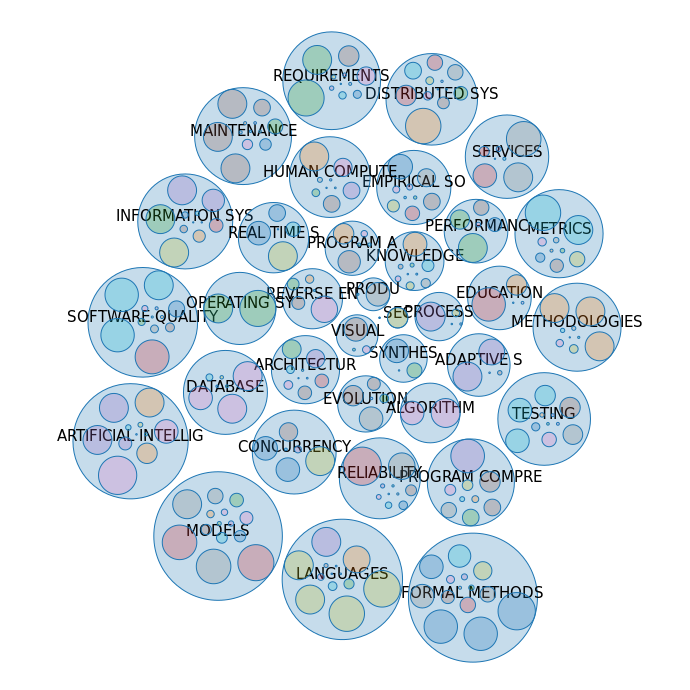
\includegraphics[width=0.80\linewidth, height=\textheight,keepaspectratio]{img/gamma-01-burbujas-alg-3.png}
	\caption{}
	\label{res:gamma01-bur-alg-3}
\end{figure}

\begin{figure}[H]
	\centering
	$HACP+T$ con $\gamma=0.1$ \\
	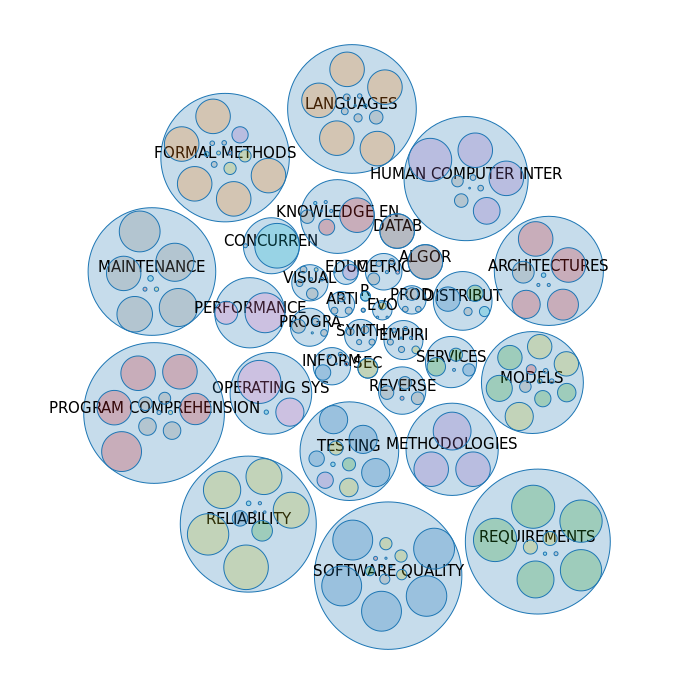
\includegraphics[width=0.80\linewidth, height=\textheight,keepaspectratio]{img/gamma-01-burbujas-alg-6.png}
	\caption{}
	\label{res:gamma01-bur-alg-6}
\end{figure}

\begin{figure}[H]
	\centering
	$BOBP$ con $\gamma=0.9$ \\
	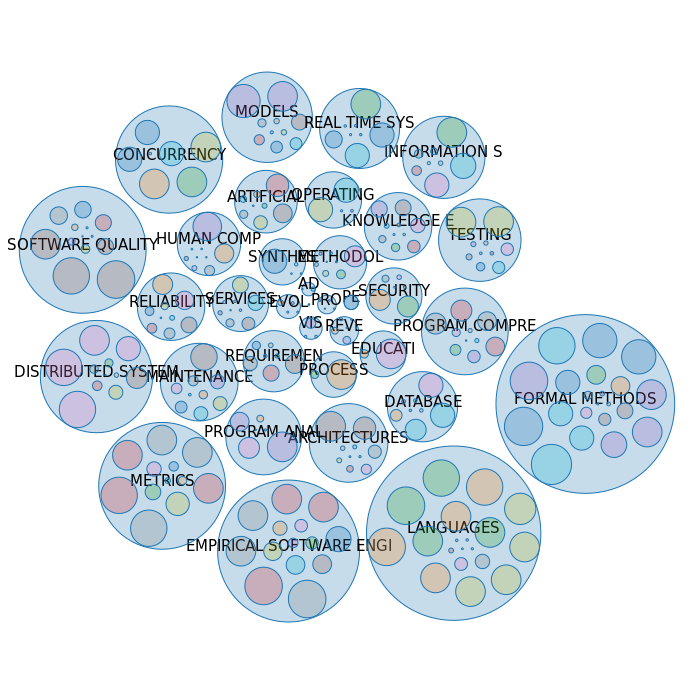
\includegraphics[width=0.80\linewidth, height=\textheight,keepaspectratio]{img/gamma-09-burbujas-alg-3.png}
	\caption{}
	\label{res:gamma09-bur-alg-3}
\end{figure}

\begin{figure}[H]
	\centering
	$HACS$ con $\gamma=0.9$ \\
	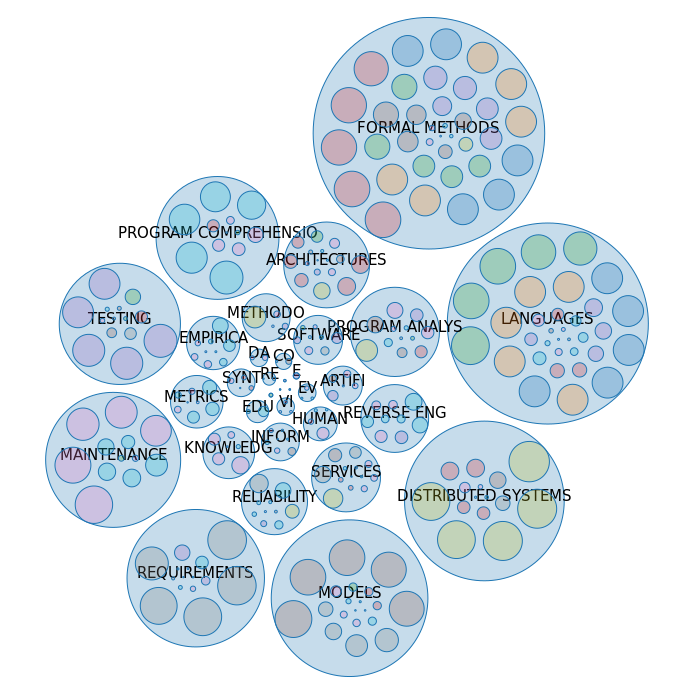
\includegraphics[width=0.80\linewidth, height=\textheight,keepaspectratio]{img/gamma-09-burbujas-alg-1.png}
	\caption{}
	\label{res:gamma09-bur-alg-1}
\end{figure}

\begin{figure}[H]
	\centering
	$BOBP$ con $\gamma=0.1$ \\
	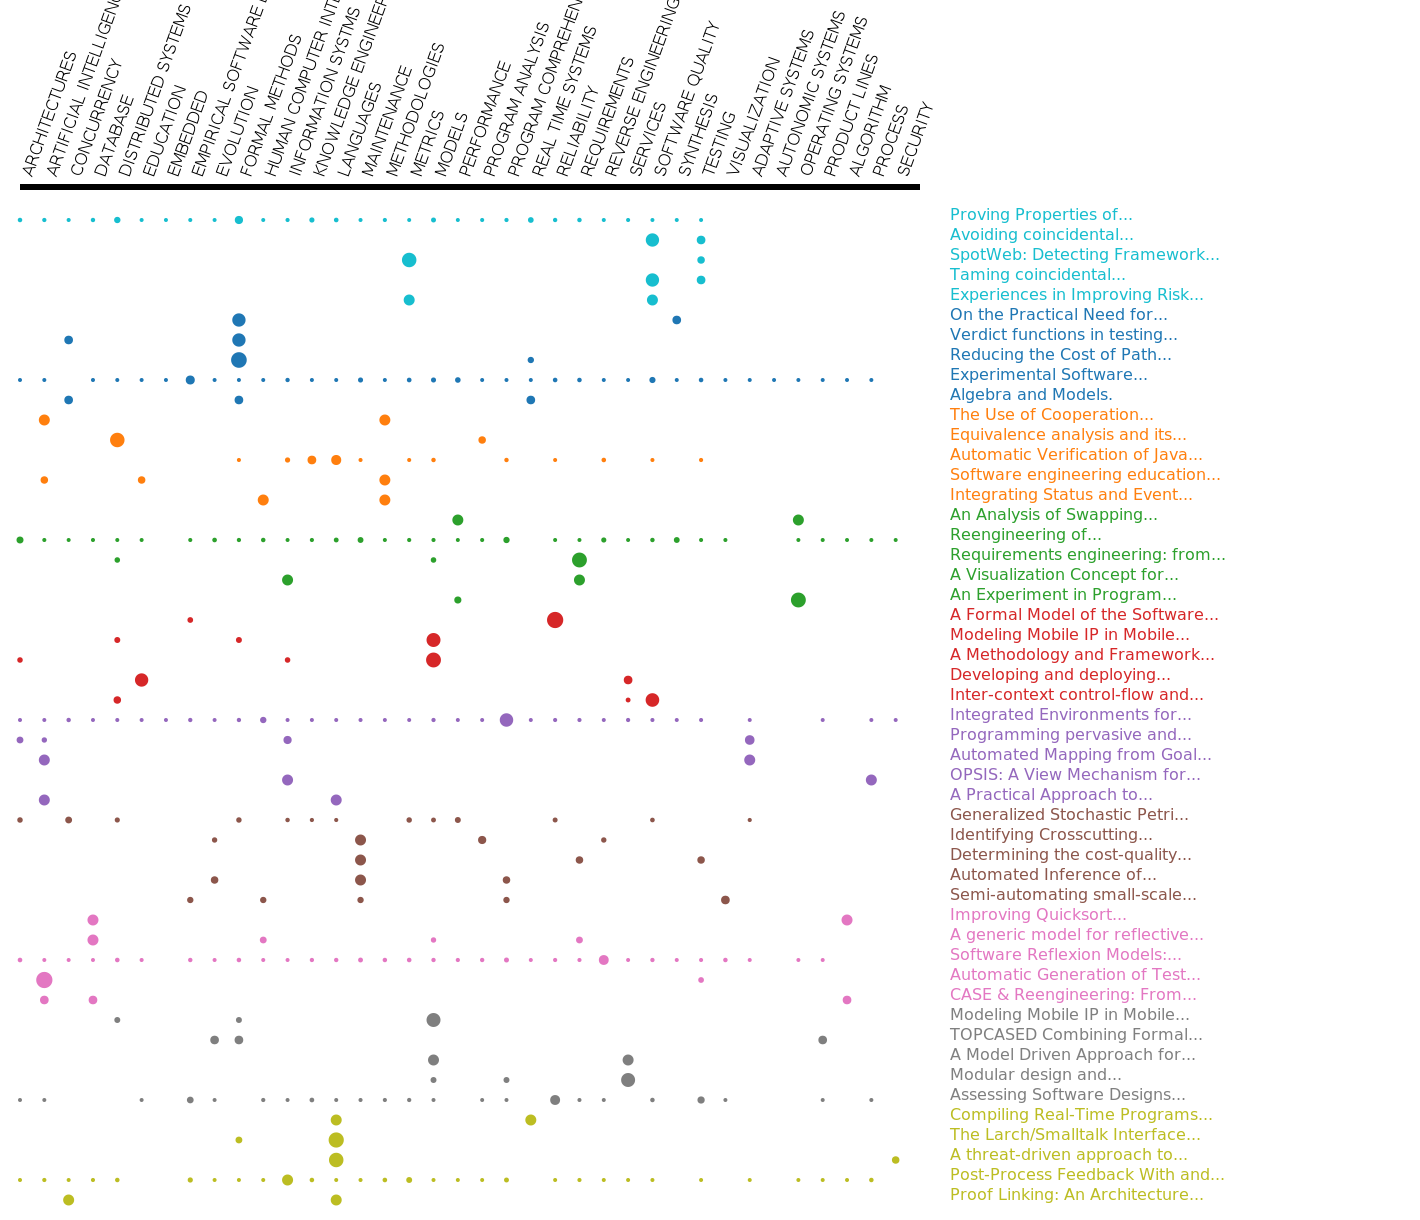
\includegraphics[width=0.80\linewidth]{img/gamma-01-alg-3.png}
	\caption{}
	\label{res:gamma01-alg-1}
\end{figure}

\begin{figure}[H]
	\centering
	$BOBP+T$ con $\gamma=0.1$ \\
	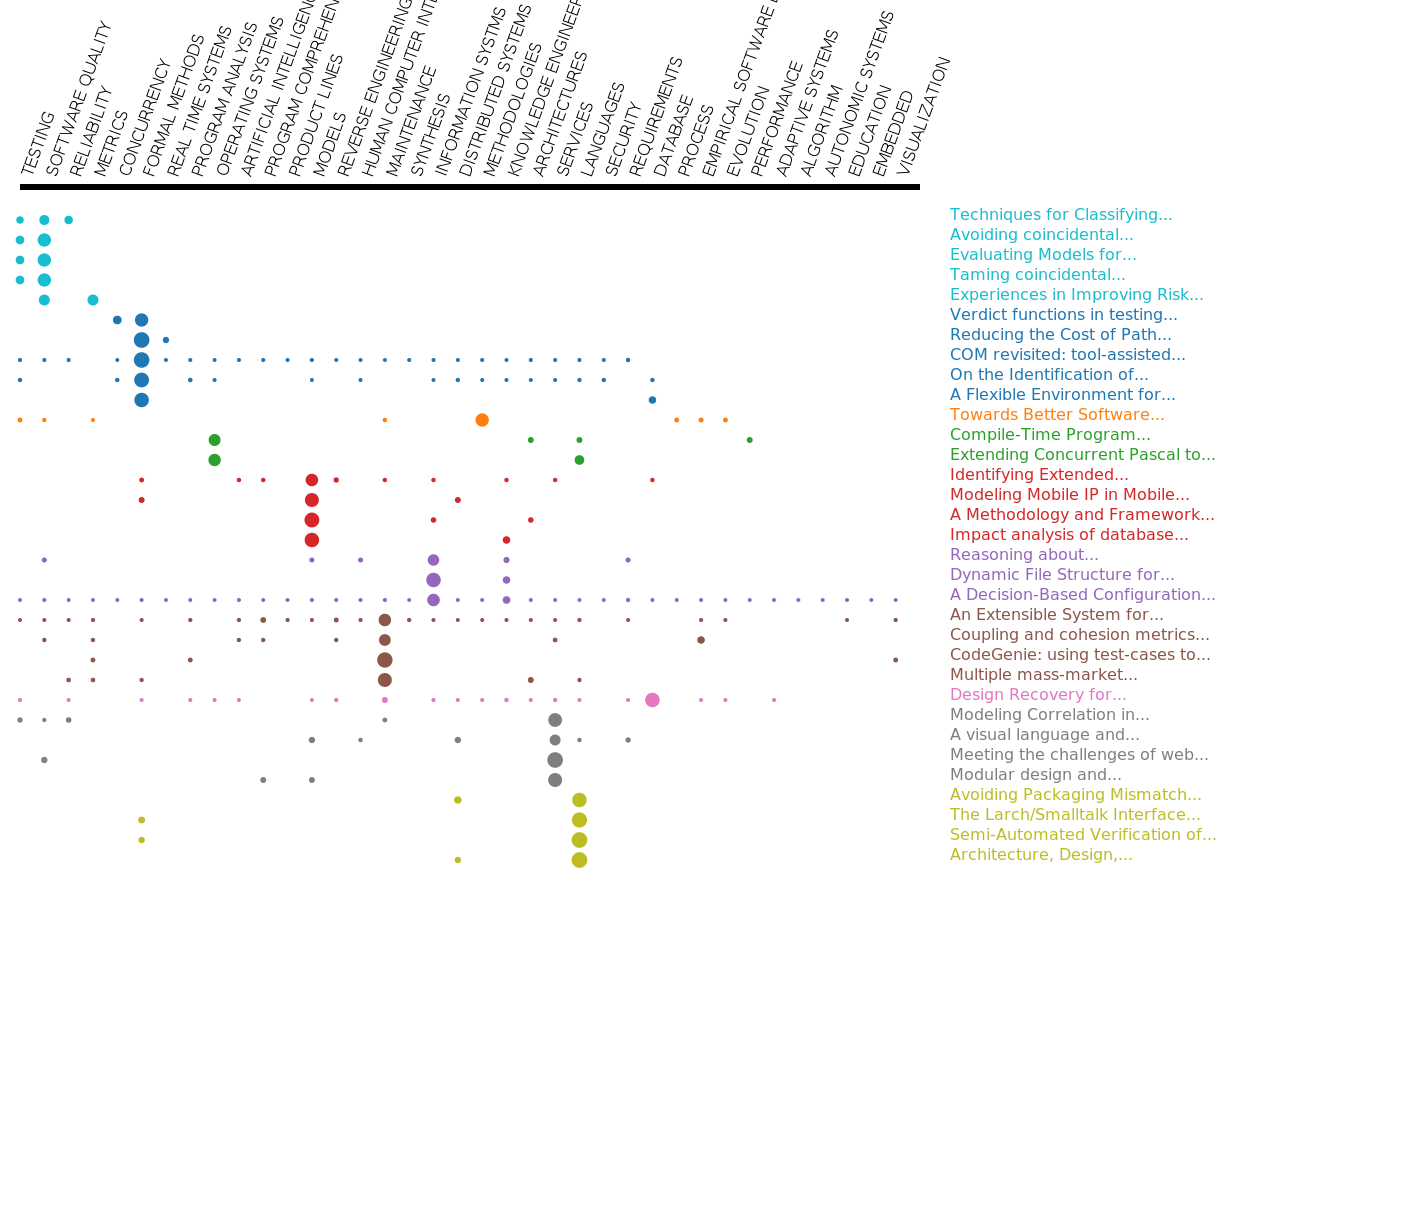
\includegraphics[width=0.80\linewidth]{img/gamma-01-alg-4.png}
	\caption{}
	\label{res:gamma01-alg-4}
\end{figure}

\begin{figure}[H]
	\centering
	$BOBOP$ con $\gamma=0.9$ \\
	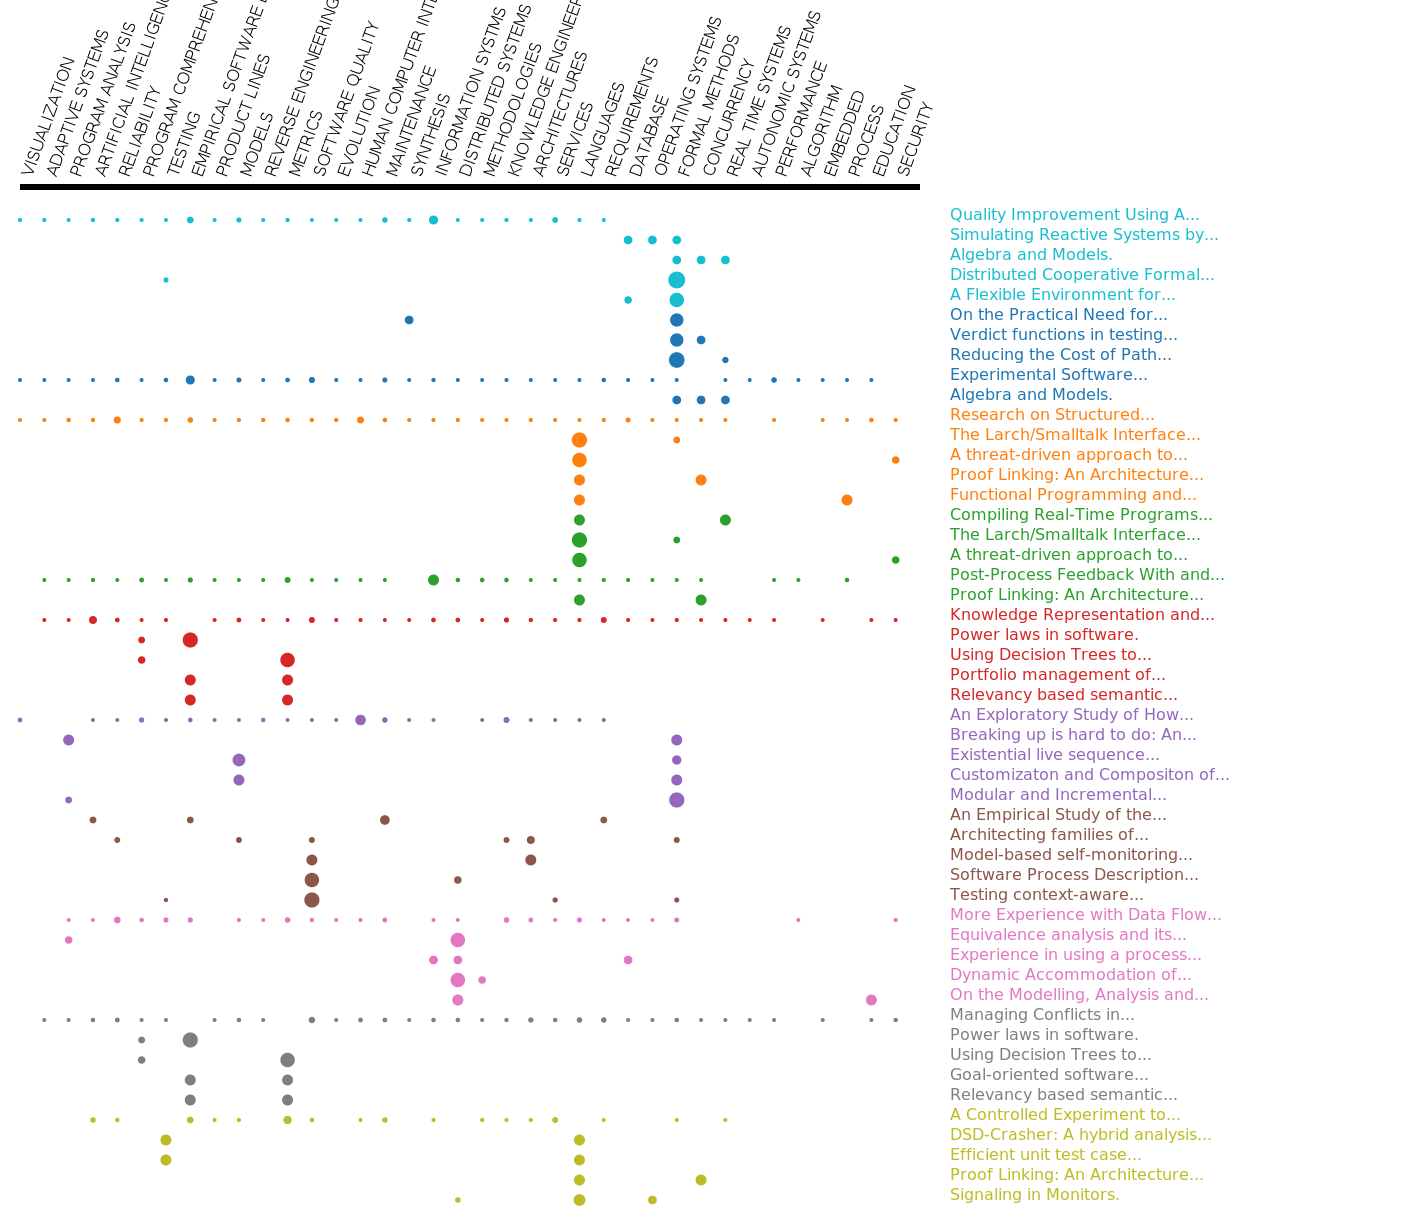
\includegraphics[width=0.80\linewidth]{img/gamma-09-alg-3.png}
	\caption{}
	\label{res:gamma09-alg-1}
\end{figure}

\begin{figure}[H]
	\centering
	$BOBOP+T$ con $\gamma=0.9$ \\
	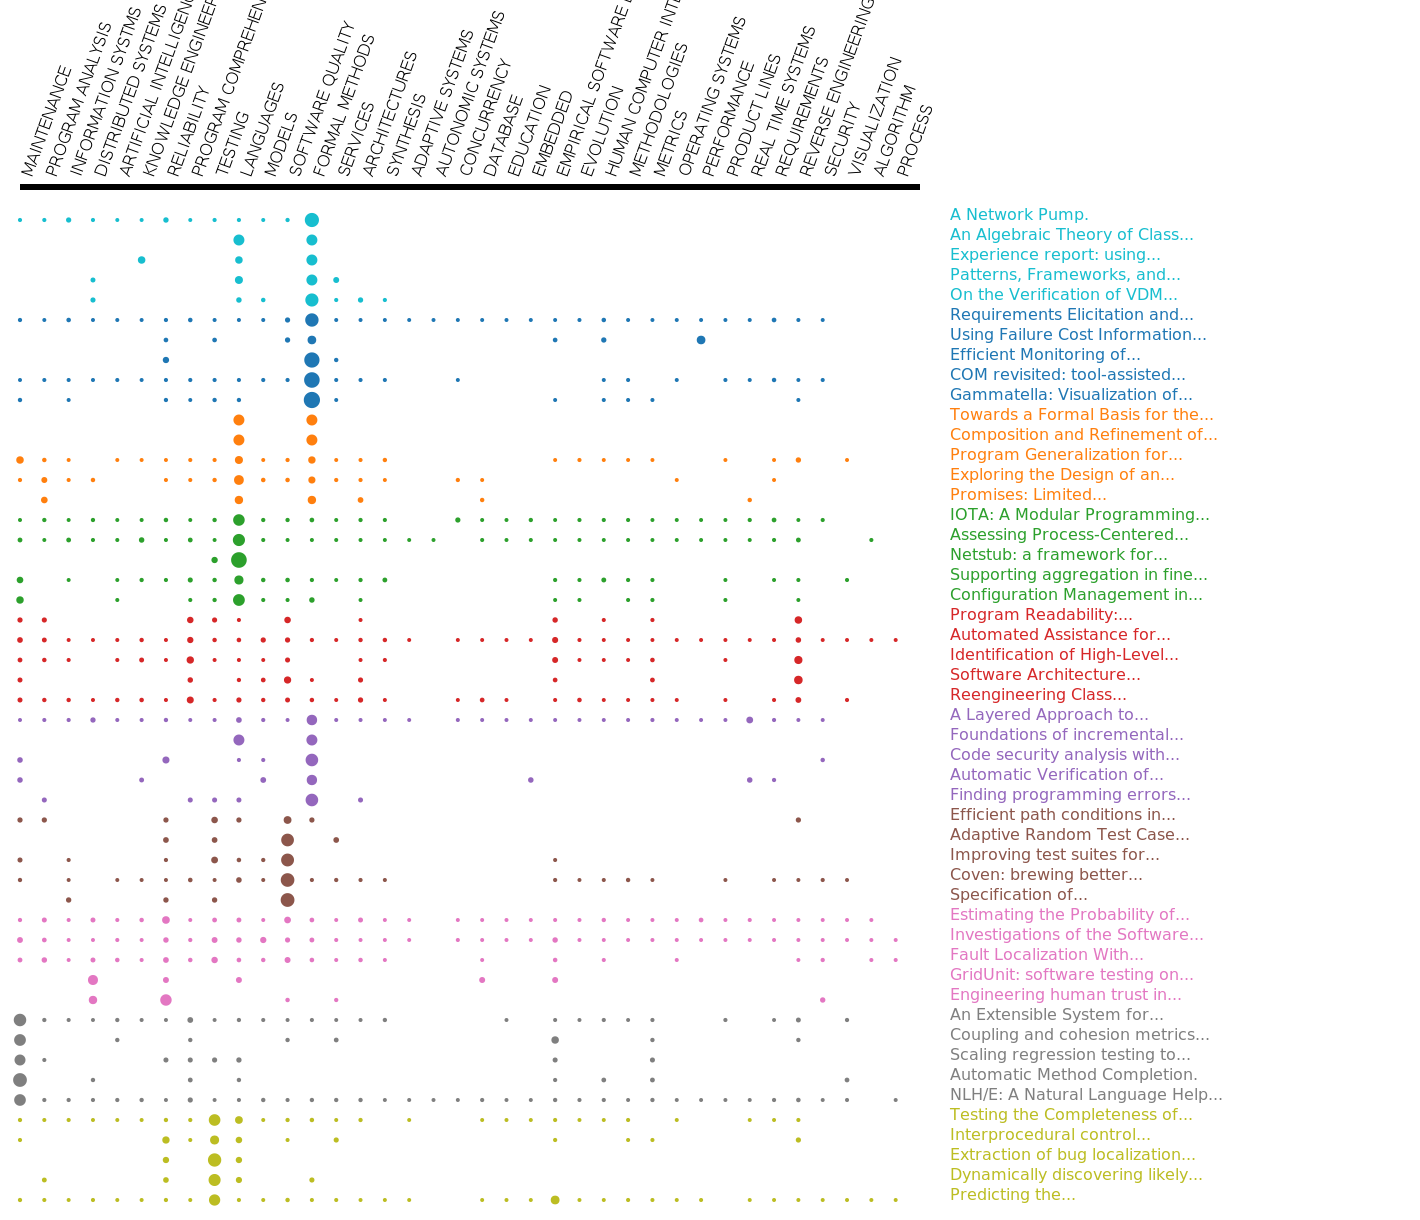
\includegraphics[width=0.80\linewidth]{img/gamma-09-alg-4.png}
	\caption{}
	\label{res:gamma09-alg-4}
\end{figure}